\section{Coding Conventions, Best Practices, and Standarization}

\subsection{PEPs}

\href{https://peps.python.org/}{Python Enhancement Proposals (PEPs)} is an online document, which is a collection of guidelines, best practices, descriptions of (new) features and implementations, as well as processes, mechanisms and important information surrounding Python. There are many PEPs, hundreds of them.

\begin{itemize}
    \item \textbf{\href{https://www.python.org/dev/peps/}{PEP 0 - Index of Python Enhancement Proposals (PEPs)}}
    \item \textbf{\href{https://www.python.org/dev/peps/pep-0001/}{PEP 1 - PEP Purpose and Guidelines:} Information about the purpose of PEPs, their types, and introduces general guidelines}
    \item \textbf{\href{https://www.python.org/dev/peps/pep-0008/}{PEP 8 - Style Guide for Python Code:} Conventions and best practices for Python coding}
    \item \textbf{\href{https://www.python.org/dev/peps/pep-0020/}{PEP 20 - The Zen of Python:} List of principles for Python’s design}
    \item \textbf{\href{https://www.python.org/dev/peps/pep-0257/}{PEP 257 - Docstring Conventions:} Provides guidelines for conventions and semantics associated with Python docstrings}
    \item \textbf{\href{https://www.python.org/dev/peps/pep-0484/}{PEP 484 - Type Hints:} Introduces a syntax for specifying type annotations in Python code}
\end{itemize}

\newpage
\subsection{PEP 1 – PEP Purpose and Guidelines}
\subsubsection{What is a PEP?}
PEP stands for Python Enhancement Proposal. A PEP is a design document providing information to the Python community, or describing a new feature for Python or its processes or environment. The PEP should provide a concise technical specification of the feature and a rationale for the feature. We intend PEPs to be the primary mechanisms for proposing major new features, for collecting community input on an issue, and for documenting the design decisions that have gone into Python. The PEP author is responsible for building consensus within the community and documenting dissenting opinions.

Because the PEPs are maintained as text files in a versioned repository, their revision history is the historical record of the feature proposal. This historical record is available by the normal git commands for retrieving older revisions, and can also be browsed on GitHub.\\

\subsubsection{PEP Audience}
The typical primary audience for PEPs are the core developers of the CPython reference interpreter and their elected Steering Council, as well as developers of other implementations of the Python language specification.

However, other parts of the Python community may also choose to use the process (particularly for Informational PEPs) to document expected API conventions and to manage complex design coordination problems that require collaboration across multiple projects.\\

\subsubsection{PEP Types}
There are three kinds of PEP:

\begin{itemize}
    \item \textbf{Standards Track PEP:} Describes a new feature or implementation for Python. It may also describe an interoperability standard that will be supported outside the standard library for current Python versions before a subsequent PEP adds standard library support in a future version.
    
    \item \textbf{Informational PEP:} Describes a Python design issue, or provides general guidelines or information to the Python community, but does not propose a new feature. Informational PEPs do not necessarily represent a Python community consensus or recommendation, so users and implementers are free to ignore Informational PEPs or follow their advice.
    
    \item \textbf{Process PEP:} Describes a process surrounding Python, or proposes a change to (or an event in) a process. Process PEPs are like Standards Track PEPs but apply to areas other than the Python language itself. They may propose an implementation, but not to Python’s codebase; they often require community consensus; unlike Informational PEPs, they are more than recommendations, and users are typically not free to ignore them. Examples include procedures, guidelines, changes to the decision-making process, and changes to the tools or environment used in Python development. Any meta-PEP is also considered a Process PEP.
\end{itemize}

\newpage
\subsection{PEP 8 – Style Guide for Python Code}

PEP 8 is a guide for writing Python code that enhances its readability and maintainability. It provides guidelines for formatting, naming conventions, code structure, and documentation.

Code is read much more often than it is written. The guidelines provided here are intended to improve the readability of code and make it consistent across the wide spectrum of Python code. As PEP 20 says, “Readability counts”.\\

\subsubsection{Key Points from PEP 8}

\begin{itemize}
    \item \textbf{Indentation:} Use 4 spaces per indentation level. Spaces are the preferred indentation method. Tabs should be used solely to remain consistent with code that is already indented with tabs. Python disallows mixing tabs and spaces for indentation.
    \item \textbf{Line Length:} Limit lines to 79 characters to enhance readability. For flowing long blocks of text with fewer structural restrictions (docstrings or comments), the line length should be limited to 72 characters.
    \item \textbf{Blank Lines:} Use blank lines to separate functions, classes, and sections of code logically.
    \item \textbf{Imports:} Import statements should be on separate lines and grouped in the following order: standard library imports, related third-party imports, and local application/library specific imports.
    \item \textbf{Whitespace:} Use whitespace to improve readability, but avoid excessive use.
    \item \textbf{Naming Conventions:} Follow naming conventions for variables, functions, and classes to maintain consistency.
    \item \textbf{Comments:} Write comments to explain non-obvious code, but avoid redundant comments.
    \item \textbf{Docstrings:} Use docstrings to document modules, functions, classes, and methods.
    \item \textbf{Coding Recommendations:} Follow best practices for coding, such as using exception handling properly and preferring exceptions to returning \texttt{None}.
    \item \textbf{Version Bookkeeping:} Use \texttt{\_\_version\_\_} for version information in modules.
        \item \textbf{Line Break Before or After Binary Operator:} It is permissible to break before or after a binary operator, as long as the convention is consistent locally. For new code it is suggested, where a line break occurs before binary operators for improved readability.
    \item \textbf{String Quotes:} Single-quoted strings and double-quoted strings are the same. This PEP does not make a recommendation for this. Pick a rule and stick to it. When a string contains single or double quote characters, however, use the other one to avoid backslashes in the string. It improves readability.
    \item \textbf{Line Continuation:} If implicit line continuation is not possible, such as when breaking a long string or expression outside of parentheses, you can use a backslash at the end of the line to indicate that it continues on the next line.
\end{itemize}

\newpage
\subsubsection{Naming Conventions}
Following naming conventions is essential for writing clean, readable, and maintainable code. Following naming conventions helps make your Python code more consistent and understandable for yourself and others who may read or work with your code.

\begin{itemize}
    \item \textbf{Variables and function names}
    \begin{itemize}
        \item Use \textbf{snake\_case}, lowercase letters with words separated by underscores for variable names and function names.
        \item Example: \texttt{my\_variable}, \texttt{calculate\_average()}
    \end{itemize}

    \item \textbf{Constants}
    \begin{itemize}
        \item Use \textbf{SCREAMING\_SNAKE\_CASE}, uppercase letters with words separated by underscores for constant names.
        \item Example: \texttt{MAX\_VALUE}, \texttt{PI}
    \end{itemize}

    \item \textbf{Class names}
    \begin{itemize}
        \item Use \textbf{CamelCase} for class names, starting with an uppercase letter.
        \item Example: \texttt{MyClass}, \texttt{Person}
    \end{itemize}

    \item \textbf{Package and module names}
    \begin{itemize}
         \item Use lowercase letters for package and module names, avoiding underscores if possible.
        \item Example: \texttt{mypackage}, \texttt{my\_module}, \texttt{utilities}, \texttt{data\_processing}
    \end{itemize}

 
\end{itemize}

\begin{figure}[h!]
    \centering
    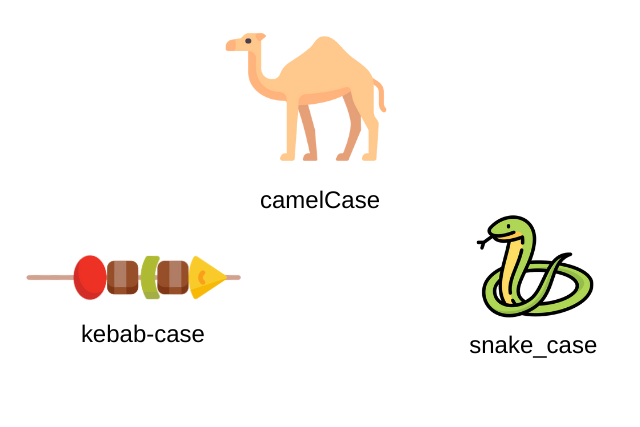
\includegraphics[width=0.6\textwidth]{images/cases2.png}
    \caption{Cases}
    \label{fig:cc-1}
\end{figure}

\newpage
\subsubsection{Comments}
\textbf{Block Comments}\\
Block comments generally apply to some (or all) code that follows them, and are indented to the same level as that code. Each line of a block comment starts with a comment marker \texttt{\#} and a single space, unless it is indented text inside the comment. Paragraphs inside a block comment are separated by a line containing a single comment marker.\\

\begin{codebox}
\begin{minted}{python}
# This is a block comment
# This function calculates the area of a circle.
# It takes the radius of the circle as input and returns the calculated area.
def calculate_area(radius):
    pi = 3.14159
    area = pi * radius ** 2
    return area
\end{minted}
\end{codebox}


\spacedtextbf{Inline comments}
\begin{itemize}
\item Use inline comments sparingly.
\item An inline comment is a comment on the same line as a statement. 
\item Should be separated by at least two spaces from the statement. 
\item They should start with a \texttt{\#} and a single space.
\item Inline comments are unnecessary and in fact distracting if they state the obvious.
\end{itemize}
%\begin{codebox}
%\begin{minted}{python}
%x = x + 1   # Increment x
%\end{minted}
%\end{codebox}


\subsubsection{Compliant Checker}
A PEP8 compliant checker is a tool used to ensure that Python code conforms to the guidelines outlined in PEP8, which is the Python Enhancement Proposal that provides conventions for writing Python code in a consistent and readable manner. PEP8 covers aspects such as indentation, line length, import formatting, naming conventions, and more.

There are several tools available for checking PEP8 compliance of Python code, including:

\begin{itemize}
    \item \textbf{pycodestyle}: Formerly known as pep8, this is a tool to check Python code against the PEP8 style guide. It can be run from the command line.
    
    \item \textbf{flake8}: Combines several tools in one package, including pycodestyle, pyflakes (for static code analysis), and McCabe (for complexity checking). It provides a comprehensive tool for checking both PEP8 compliance and potential errors in your code.
    
    \item \textbf{Black}: While not strictly a PEP8 checker, Black is a code formatter that automatically reformats Python code to comply with PEP8 standards. It enforces a consistent style by rewriting code to adhere to its strict rules.
    
    \item \textbf{PyLint}: Another popular tool for analyzing Python code for errors, it also provides checks for PEP8 compliance among other things.
\end{itemize}

\newpage
\subsection{PEP 20 – The Zen of Python}

PEP 20 is titled "The Zen of Python" and was authored by Tim Peters. It serves as a set of guiding principles or philosophies for the design of the Python programming language. It encapsulates the core values and ideals that Python's creators and community strive to uphold in their programming practices. The aphorisms, or principles, outlined in PEP 20 are:\\

\begin{itemize}
    \item Beautiful is better than ugly.
    \item Explicit is better than implicit.
    \item Simple is better than complex.
    \item Complex is better than complicated.
    \item Flat is better than nested.
    \item Sparse is better than dense.
    \item Readability counts.
    \item Special cases aren't special enough to break the rules.
    \item Although practicality beats purity.
    \item Errors should never pass silently.
    \item Unless explicitly silenced.
    \item In the face of ambiguity, refuse the temptation to guess.
    \item There should be one-- and preferably only one --obvious way to do it.
    \item Although that way may not be obvious at first unless you're Dutch.
    \item Now is better than never.
    \item Although never is often better than \textit{right} now.
    \item If the implementation is hard to explain, it's a bad idea.
    \item If the implementation is easy to explain, it may be a good idea.
    \item Namespaces are one honking great idea -- let's do more of those!
\end{itemize}

\subsubsection{Easter Egg: \texttt{import this}}
The term "Easter Egg" refers to a hidden feature or message that developers embed within the code for amusement or as a tribute. The term is derived from the tradition of hiding Easter eggs for children to find during Easter egg hunts.\\

The code snippet "\texttt{import this}" is a well-known Easter Egg. When executed in a Python interpreter, it displays "The Zen of Python," which is a collection of aphorisms that capture the guiding principles of Python's design philosophy. These aphorisms were written by Tim Peters, and they provide insights into the mindset and values of Python developers.

%\begin{figure}[h]
%    \centering
%    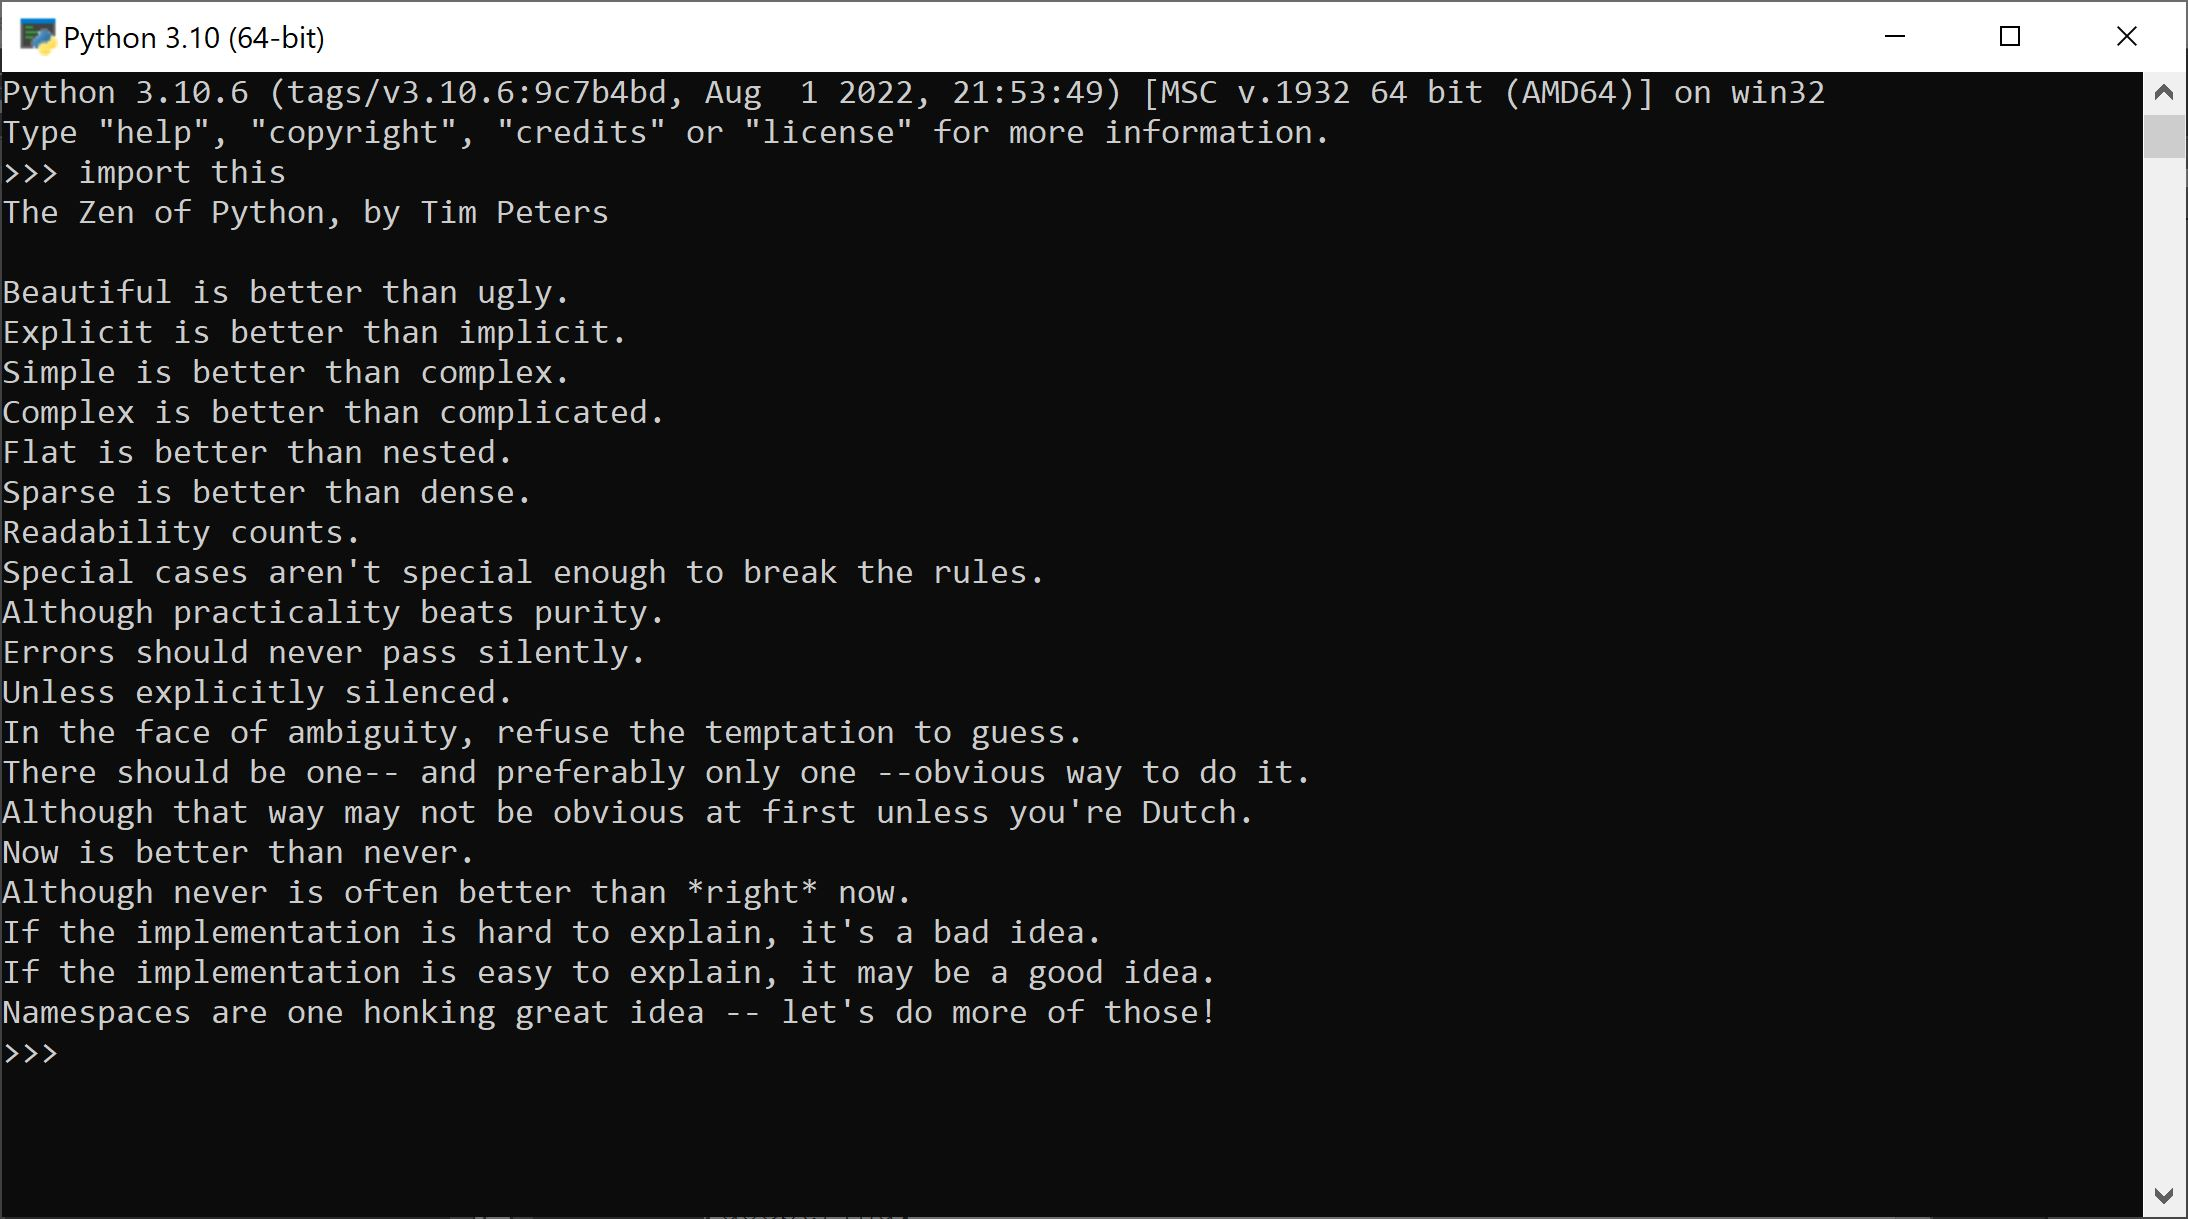
\includegraphics[width=\textwidth]{images/import_this.JPG}
%    \caption{import this}
%    \label{fig:example}
%\end{figure}

\newpage
\subsection{PEP 257 – Docstring Conventions}
PEP 257 provides conventions for writing docstrings. Docstrings are documentation strings that appear as the first statement in a module, function, class, or method definition. The key points from PEP 257 are:

\begin{itemize}
    \item Docstrings should be enclosed in triple quotes, e.g. \texttt{"""This is a docstring."""}.
    \item For a multi-line docstring, the opening and closing quotes should be on separate lines.
    \item The first line of a docstring should be a summary of the object's purpose, starting with a capital letter and ending with a period.
    \item If the docstring has multiple paragraphs, subsequent paragraphs should be separated by a blank line.
    \item Docstrings should be written in complete sentences and follow proper grammar and punctuation rules.
    \item Docstrings should include information about the function or method's parameters, return values, exceptions raised, and any side effects.
    \item For module-level docstrings, they should include an overview of the module's contents and usage examples.
    \item For class docstrings, they should describe the class's purpose, behavior, and usage, including information about constructor arguments and instance variables.
\end{itemize}

\subsubsection{One-line Docstrings}
One-liners are for really obvious cases. They should really fit on one line.
\begin{codebox}
\begin{minted}{python}
def kos_root():
    """Return the pathname of the KOS root directory."""
    global _kos_root
    if _kos_root: return _kos_root
    ...
\end{minted}
\end{codebox}

\begin{itemize}
    \item Triple quotes are used even though the string fits on one line. Makes it easy to expand it.
    \item The closing quotes are on the same line as the opening quotes. Looks better for one-liners.
    \item There’s no blank line either before or after the docstring.
    \item The docstring is a phrase ending in a period. It prescribes the function or method’s effect as a command (“Do this”, “Return that”), not as a description; e.g. don’t write “Returns the pathname …”.
    \item The one-line docstring should NOT be a “signature” reiterating the function/method parameters (which can be obtained by introspection).
\end{itemize}

\newpage
\subsubsection{Multi-line Docstrings}
Multi-line docstrings consist of a summary line just like a one-line docstring, followed by a blank line, followed by a more elaborate description. The summary line may be used by automatic indexing tools; it is important that it fits on one line and is separated from the rest of the docstring by a blank line. The summary line may be on the same line as the opening quotes or on the next line. The entire docstring is indented the same as the quotes at its first line (see example below).
\begin{codebox}
\begin{minted}{python}
def complex(real=0.0, imag=0.0):
    """Form a complex number.

    Keyword arguments:
    real -- the real part (default 0.0)
    imag -- the imaginary part (default 0.0)
    """
    if imag == 0.0 and real == 0.0:
        return complex_zero
    ...
\end{minted}
\end{codebox}

\subsubsection{Linters and Fixers}
Linters and fixers are tools used in software development to analyze source code for potential errors, bugs, stylistic inconsistencies, and adherence to coding standards. They automate the process of code review by identifying issues and providing feedback to developers, helping ensure code quality, consistency, and maintainability.\\

\begin{itemize}
\item \textbf{Linter}
\begin{itemize}
    \item Static code analysis tool used to flag programming errors, bugs, stylistic errors, and suspicious constructs in the source code without actually executing it.
    \item Maintain a consistent coding style within a project and can catch common programming mistakes early in the development process.
    \item Commonly used in software development to improve code quality, readability, and maintainability.
\end{itemize}

\item \textbf{Fixer}
\begin{itemize}
    \item Tool that automatically corrects or adjusts code based on the suggestions and warnings provided by a linter.
    \item Automatically apply changes to the code, such as formatting corrections, removing unused imports, or fixing syntax errors.
    \item Streamline the development process by automating repetitive tasks and ensuring that the codebase adheres to the defined coding standards.
\end{itemize}
\end{itemize}


\newpage
\subsection{PEP 484 – Type Hints}
In Python, "types" refer to the classification of data into different categories, such as integers, strings, lists, etc. Python is known for its dynamic typing system, which means that the type of a variable is inferred at runtime based on the value it holds. This is in contrast to statically typed languages like Java or C++, where you must declare the type of a variable explicitly.

\subsubsection{Dynamic Typing}
Python's dynamic typing offers flexibility and simplicity, allowing developers to write code more quickly and concisely. However, it also means that type errors may only be discovered at runtime, leading to potential bugs that can be harder to catch during development.\\

To address this issue, Python introduced optional static typing through PEP 483 and PEP 484. These proposals introduced type hints, a syntax for annotating variables, function parameters, and return values with their expected types. 
%Although these annotations are not enforced by the Python interpreter at runtime, they can be used by static analysis tools, such as MyPy, to perform type checking and catch potential errors early in the development process.

\begin{codebox}
\begin{minted}{python}
# Import the typing module for type hints
from typing import List

# Type hints for variables
age: int = 30
names: List[str] = ["Alice", "Bob", "Charlie"]

# Functions with type hints for parameters and return value
def greet(name: str) -> str:
    return f"Hello, {name}"

def upper_everything(elements: list[str]) -> list[str]:
    return [el.upper() for el in elements]
\end{minted}
\end{codebox}

\subsubsection{Type Checker: Mypy}
Mypy is an optional static type checker for Python that aims to combine the benefits of dynamic (or "duck") typing and static typing. Mypy combines the expressive power and convenience of Python with a powerful type system and compile-time type checking. Mypy type checks standard Python programs; run them using any Python VM with basically no runtime overhead.\\

Using mypy alongside your Python development workflow can help catch type-related errors early, improve code maintainability, and enhance collaboration, especially in larger projects or teams where type clarity is beneficial.

\begin{codebox}
\begin{minted}{bash}
# Install mypy
pip install mypy

# Run mypy on a single Python script or module
mypy your_script.py

# Run mypy on an entire directory (recursively)
mypy your_directory/
\end{minted}
\end{codebox}

